\chapter{The Syntax of the Input File}

Most of the functionality of \linnet{} is controlled from the input file.
The main part of the input file is the circuit netlist: Each line of code
defines a single electronic device with the network nodes it is connected
to. The number of nodes varies from two to four and depends on the kind of
device. Nodes are defined implicitly the first time they are referenced by
a device definition.

The remaining parts of the file are used to specify the wanted results.
This part of the file may stay empty, in which case all unknown quantities
are computed.


\section{Basic syntax elements}

A netlist file may of course be well-documented. You can use C/C++ style
comments anywhere. Nested comments are not supported.

A semicolon is treated like an end of line character. Line concatenation
can be achieved with a backslash as very last character of a line, as in
the language C.

All elements of the formal syntax of the input file are treated case
sensitive.

The names of devices, nodes, user-defined voltages and results are defined
as identifiers in most computer languages. They begin with a letter or
underscore and can continue with any number of the same or decimal digits.
This particularly disables integer numbers to become node designations as
it is common in SPICE netlists.

The names of knowns and unknowns are internally derived from the device
and node names and are in turn ``identifiers''. 


\begin{longtable}{|c|c|c|}

\hline
\label{tabExponentSuffixes}
% The column headers (first page):
Suffix & Meaning & Value \\ \hline
% This hline makes the column titles a separate rectangular box, comment out to get just a
% line as separator.
%\hline
\endfirsthead

\hline
% The column headers (other pages):
Suffix & Meaning & Value \\ \hline
% This hline makes the column titles a separate rectangular box, comment out to get just a
% line as separator.
%\hline
\endhead

\hline
\caption{Suffixes for exponents in floating point literals (continued on next page)} 
\endfoot

\hline
\caption{Suffixes for exponents in floating point literals}
\endlastfoot

\hline

% Table entries start here.
\code{y} & yocto & \raisebox{0pt}[10pt][0pt]{$10^{-24}$} \\
\code{z} & zepto & \raisebox{0pt}[10pt][0pt]{$10^{-21}$} \\ 
\code{a} & atto  & \raisebox{0pt}[10pt][0pt]{$10^{-18}$} \\ 
\code{f} & femto & \raisebox{0pt}[10pt][0pt]{$10^{-15}$} \\ 
\code{p} & pico  & \raisebox{0pt}[10pt][0pt]{$10^{-12}$} \\ 
\code{n} & nano  & \raisebox{0pt}[10pt][0pt]{$10^{-9}$}  \\ 
\code{u} & micro & \raisebox{0pt}[10pt][0pt]{$10^{-6}$}  \\ 
\code{m} & milli & \raisebox{0pt}[10pt][0pt]{$10^{-3}$}  \\ 
\code{c} & centi & \raisebox{0pt}[10pt][0pt]{$10^{-2}$}  \\ 
\code{d} & deci  & \raisebox{0pt}[10pt][0pt]{$10^{-1}$}  \\ 
\code{D} & deka  & \raisebox{0pt}[10pt][0pt]{$10^{1}$}   \\ 
\code{h} & hecto & \raisebox{0pt}[10pt][0pt]{$10^{2}$}   \\ 
\code{k} & kilo  & \raisebox{0pt}[10pt][0pt]{$10^{3}$}   \\ 
\code{M} & mega  & \raisebox{0pt}[10pt][0pt]{$10^{6}$}   \\ 
\code{G} & giga  & \raisebox{0pt}[10pt][0pt]{$10^{9}$}   \\ 
\code{T} & tera  & \raisebox{0pt}[10pt][0pt]{$10^{12}$}  \\ 
\code{P} & peta  & \raisebox{0pt}[10pt][0pt]{$10^{15}$}  \\ 
\code{X}\footnote{According to
http://searchstorage.techtarget.com/definition/Kilo-mega-giga-tera-peta-and-all-that,
as of Feb 9, 2014, exa should be abbreviated with \code{E}. This is
ambiguous with the traditional form of an exponent. \code{1E+2} could be
either $10^{18}+2$ or $100$. We use \code{X} instead.}
         & exa   & \raisebox{0pt}[10pt][0pt]{$10^{18}$}  \\
\code{Z} & zetta & \raisebox{0pt}[10pt][0pt]{$10^{21}$}  \\ 
\code{Y} & yotta & \raisebox{0pt}[10pt][0pt]{$10^{24}$}  \\ 

\end{longtable}

Numbers are either decimal integer literals as known from the language C
or floating point numbers, depending on the context. Floating point numbers
can be written as known from the language C. For convenience, the exponent
may be abbreviated by a suffix character; just type this single character
instead of the conventional exponent expression, write for example
\code{5.6k} instead of \code{5.6e3}. Careful, the suffixes are case
sensitive, too, \code{5.6K} would yield a syntax error. The supported
suffixes are listed in table \ref{tabExponentSuffixes}

More details on the syntax definition can be found in file
\file{parser-cnl-bnf.txt}. The syntax is presented in commented
Backus-Naur form. The file is printed in appendix \ref{secBNFOfCnl} on
page \pageref{secBNFOfCnl} of this document and it is part of the
\linnet{} sources.


\section{The actual netlist}

The main part of the input file is a list of device definitions. Each
definition is placed on a new line or a semicolon is used to seperate two
definitions on the same line. A device definition starts with the device
type that indicates the kind of device. Table \ref{tabSupportedDevices} on
page \pageref{tabSupportedDevices} gives an overview on the available
devices. The type identifier from table column ID is used as first token
of a device definition in the netlist file.

The name of the device follows after some white space. All names need to
be unique in order to avoid ambiguities in the result presentation. Then
the names of the nodes the device is connected to follow up as a blank
separated list. The kind of device determines the required number of
nodes, see below.\footnote{The syntax format defines the nodes by position
in the line only. If a node name is missing in the line the next token
will be taken as this node and a missleading error message can result.
Which might be particularly confusing if it is not the last node, which
has been omitted.} There's no explicit definition of nodes; a node is
defined implicitly when referencing it in a device definition the very
first time. This doesn't hold for the voltage sensing inputs of a voltage
controlled source (the third and forth node in the device definition).
They are pure references to a pair of nodes, which need to be defined
elsewhere. Normally the parser doesn't support forward references but here
we have one of the few exceptions; the actual definition of the the source
controlling nodes may be made with a later device definition:

% Wrap text after line 87 in the verbatiom section.
\begin{verbatim}
/* This system has the input impedance Ri and an output voltage, which is the k-fold
   of the input voltage. */
U(U) k out gnd in gnd // Voltage controlled voltage source k is defined. Nodes out and
                      // gnd are implicitly defined. Nodes in and gnd are referenced;
                      // node in is not yet defined, we have a forward reference.
R Ri in gnd           // Resistor Ri is defined. Node in is implicitly defined and the
                      // above forward reference can be resolved.
U Ui in gnd           // The input voltage is modeled by a constant voltage source
\end{verbatim}

An optional blank separated device relation may follow the node
references. The device relation supports numeric post-processing and
simplifications of the final result. The simplest form of a device
relation is the assignment of a numeric value. Such an assignment has no
impact on \linnet's computation, it is solely passed on to Octave for
numeric evaluation via the generated script code. An example would be

\begin{verbatim}
R R1 k0 k1 R1=5.6k
\end{verbatim}

\noindent
which defines the resistor \code{R1}, connects it to the two nodes
\code{k0} and \code{k1} and assigns it a value of 5600\,$\Omega$. The
generated Octave script code will initialize the variable \code{R1} with
the numeric value $5600.0$. All variables which no user-defined values are
found for in the netlist file will get fixed standard values as initial
values in the generated Octave script code. The standard values are
defined such that the characteristic time constants of the circuit are
probably in the audio frequency range. Changing these standard values to
more appropriate values can then be done on the Octave command line. The
hardcoded standard values of all affected devices are listed in table
\ref{tabDeviceStdValues} on page \pageref{tabDeviceStdValues}.

More important than value assignments are relations between devices of
same kind. The most simple case would be the identity of the values of two
devices, e.g. \code{R1=R2}. Many circuits depend on such a relation; a
voltage divider with two identical resistors is for example often used to
pin the input voltage of an op-amp to half the operational voltage. If a
pair of devices has a fixed value relation as a principle of operation of
the circuit then this should be expressed in the netlist. The knowledge
about value relations enables \linnet{} to perform according
simplifications of the final result, it would e.g. simplify a term like
$R_1 R_2 C$ to ${R_2}^2 C$ in the previous example. An impressive example
of such simplifications is found as \file{octagon.cnl} in the set of test
cases in the source code distribution of \linnet{}.

Device relations can be made recursively. The netlist\footnote{The tokens
\code{DEF} and \code{RES} are explained below in section
\ref{secResultSpec}.}

\begin{verbatim}
U Uin in gnd
R R1 in k1
R R2 k1 k2  R2=R1
R R3 k2 k3  R3=R2
R R4 k3 gnd R4=R3
DEF Uout k3 gnd
RES VDiv Uout
\end{verbatim}

\noindent
defines a voltage divider into four identical voltages. Due to the given
relations, the result formula will no longer contain any device symbol,
but simply states $\frac{1}{4}U_{in}$ for the output voltage.

Device relations can use rational ratios. We could achieve the same result
with the following netlist:

\begin{verbatim}
U Uin in gnd
R R1 in k1
R R2 k1 gnd R2=1/3*R1
DEF Uout k1 gnd
RES VDiv Uout
\end{verbatim}

\linnet{} claims to be a symbolic not a numeric program. Such a software
is expected to produce exact, error free results only. Permitting rational
ratios between two devices introduces some numeric calculations but these
can still be carried out error free -- with the exception of overflows.
Making intensive use of such relations will easily produce such an
overflow. \linnet{} will recognize the overflow but not perform any
approximative computations. You either get an accurate result or no result
(but the error message). The danger of an overflow rises if you use ratios
of large numbers that are prime to each other or if you use recursive
device ratios as in the next example, which again has the same output
voltage:

\begin{verbatim}
U Uin in gnd
R R1 in k1
R R2 k1 k2  R2=(7/8)*R1
R R3 k2 gnd R3=(5/7)*R2
DEF Uout k2 gnd
RES VDiv Uout
\end{verbatim}

\noindent
To reduce the danger of overflows due to careless use of the rational
ratios the values of numerator and denominator of the ratios are limited
to the range $1..999$. Null and negative ratios are generally not
permitted. Negative ratios can be useful with controlled sources; if so
the appropriate sign has to be chosen by the polarity of either the source
or the control voltage or current.

Device relations must not use forward references. 

The definition of the device is closed with either a newline character or
semicolon. Newline characters must not be used to spread a device
definition over several lines but several device definitions can share the
same line if the semicolon is used.


\subsection{Which nodes to connect to}

% The schematics used as examples in this section are placed at the
% begining of the source code section in order to give LaTeX room to
% distribute them over all pages.

% Sample circuit: Current probe and current controlled current source
{
% This define is related to the specifics of the array package; see
% http://texwelt.de/wissen/fragen/3401/zentrieren-text-in-tabelle (as of
% July 25 2014) for more
\newcolumntype{M}[1]{>{\centering\arraybackslash}m{#1}}

\begin{figure}[t]
\begin{center}
% The standard total width of 11cm leads here to an ugly gap between
% netlist and schematic. We reduce it by 1cm.
\begin{tabular}{M{5.42cm}M{4.58cm}}
\verbatiminput{simpleT.cnl}
&
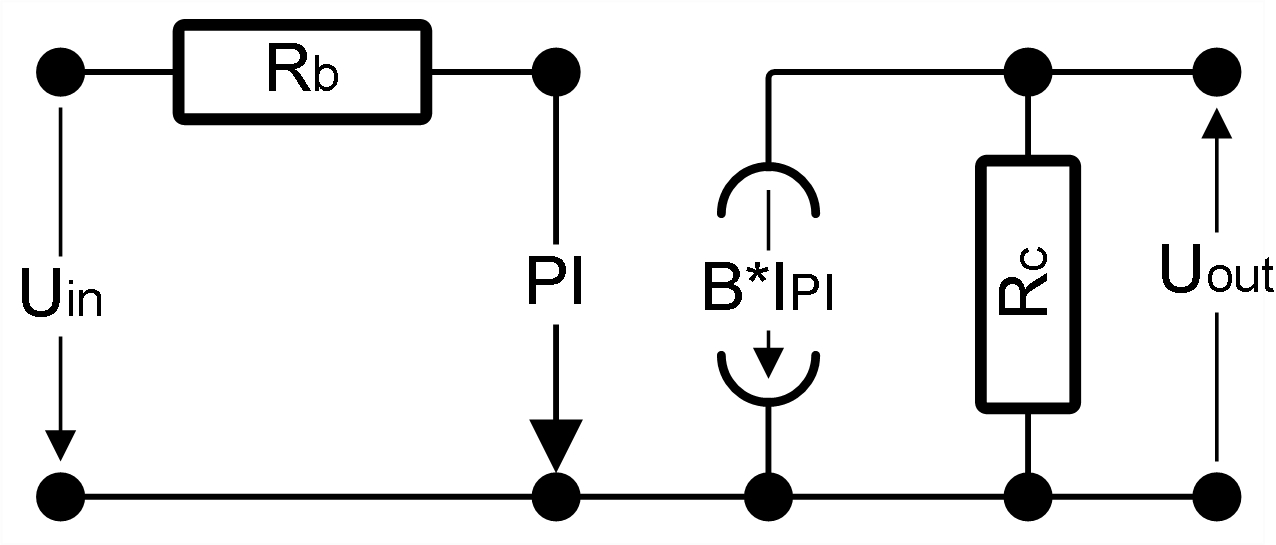
\includegraphics[width=4.58cm]{SimpleT}
\\

\end{tabular}
\caption{A simple bipolar transistor simulation}
\label{figSimpleT}
\end{center}
\end{figure}
} % End of sample circuit: Current probe and current controlled current source

% Sample circuit: The non inverting op-amp.
{
% This define is related to the specifics of the array package; see
% http://texwelt.de/wissen/fragen/3401/zentrieren-text-in-tabelle (as of
% July 25 2014) for more
\newcolumntype{M}[1]{>{\centering\arraybackslash}m{#1}}

\begin{figure}[b]
\begin{center}
\begin{tabular}{M{5.84cm}M{5.16cm}}
\verbatiminput{NonInvertingOP.cnl}
&
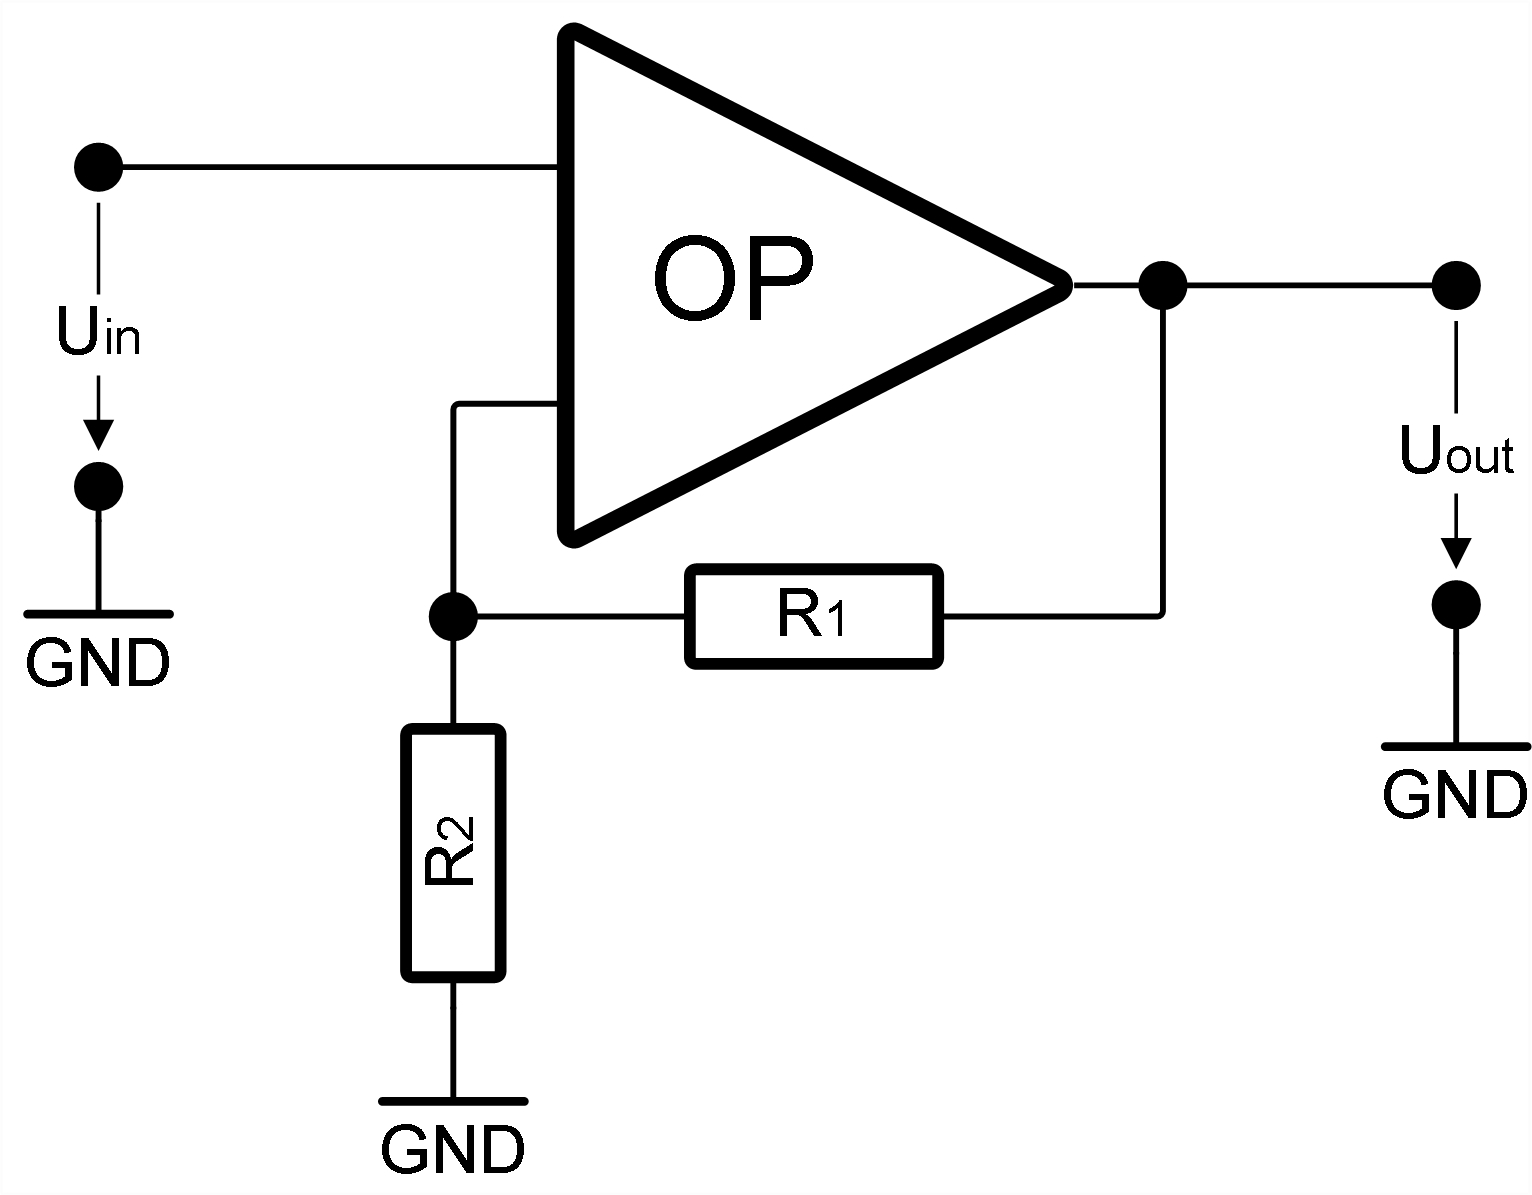
\includegraphics[width=5.16cm]{NonInvertingOP}
\\

\end{tabular}
\caption{Non inverting op-amp}
\label{figNonInvOp}
\end{center}
\end{figure}
} % End of sample circuit: The non inverting op-amp.

% Sample circuit: Model of inverting op-amp.
{
% This define is related to the specifics of the array package; see
% http://texwelt.de/wissen/fragen/3401/zentrieren-text-in-tabelle (as of
% July 25 2014) for more
\newcolumntype{M}[1]{>{\centering\arraybackslash}m{#1}}

\begin{figure}[t]
\begin{center}
\begin{tabular}{M{6.65cm}M{4.35cm}}
\verbatiminput{ModelOfOP.cnl}
&
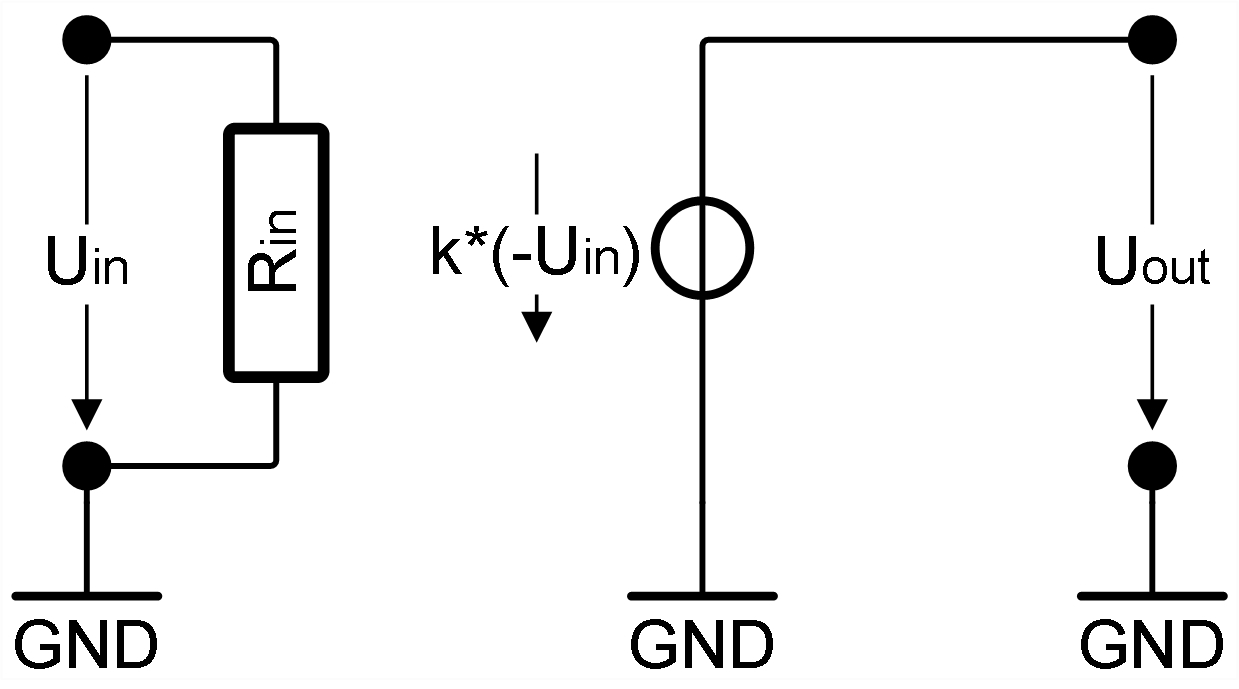
\includegraphics[width=4.35cm]{ModelOfOP}
\\

\end{tabular}
\caption{Model of the inverting op-amp}
\label{figModelOfOP}
\end{center}
\end{figure}
} % End of sample circuit: Model of inverting op-amp.

% Sample circuit: Current controlled voltage source
{
% This define is related to the specifics of the array package; see
% http://texwelt.de/wissen/fragen/3401/zentrieren-text-in-tabelle (as of
% July 25 2014) for more
\newcolumntype{M}[1]{>{\centering\arraybackslash}m{#1}}

\begin{figure}[b]
\begin{center}
\begin{tabular}{M{5.73cm}M{5.27cm}}
\verbatiminput{I2UConverter_U(i).cnl}
&
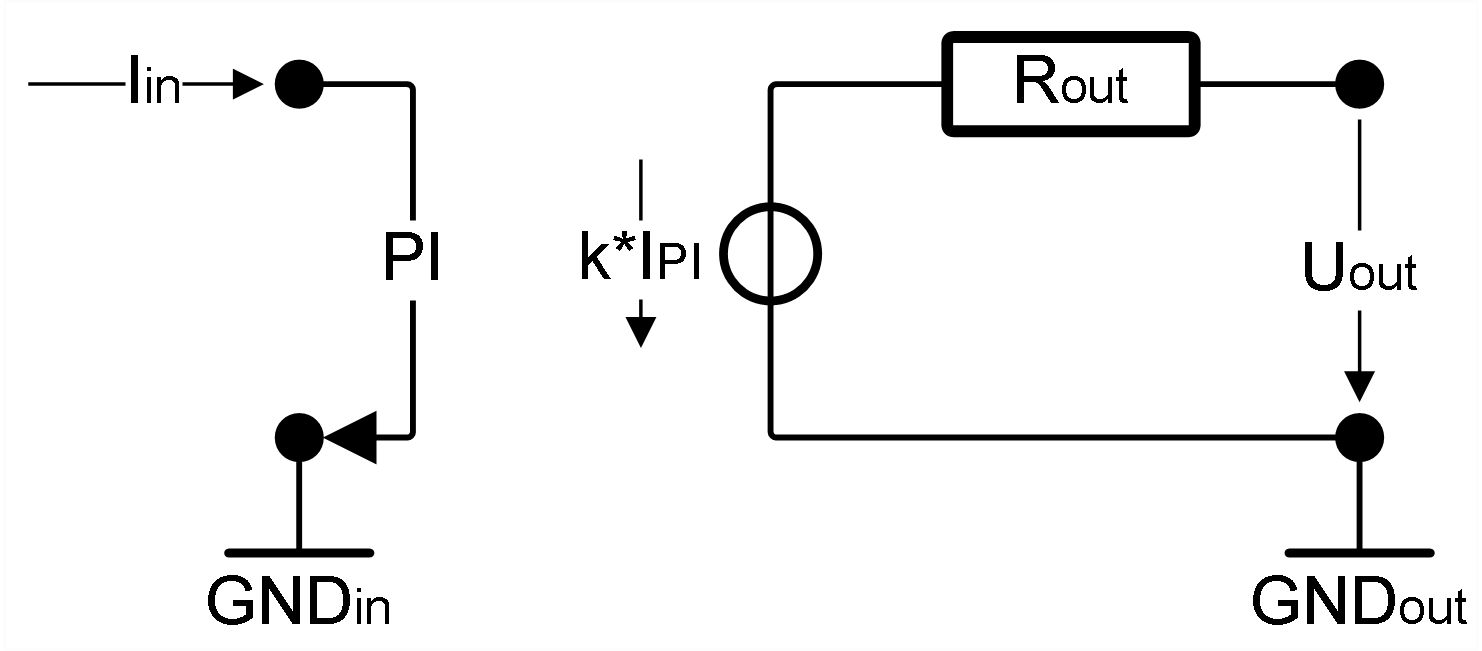
\includegraphics[width=5.27cm]{I2UConverter_U(i)}
\\

\end{tabular}
\caption{Current to voltage converter using a current controlled voltage source; $R_i=0$,
$R_o=R_{out}$}
\label{figI2UConverterUsingUByI}
\end{center}
\end{figure}
} % End of sample circuit: Current controlled voltage source

% Sample circuit: Voltage controlled current source
{
% This define is related to the specifics of the array package; see
% http://texwelt.de/wissen/fragen/3401/zentrieren-text-in-tabelle (as of
% July 25 2014) for more
\newcolumntype{M}[1]{>{\centering\arraybackslash}m{#1}}

\begin{figure}[tb]
\begin{center}
\begin{tabular}{M{5.62cm}M{5.38cm}}
\verbatiminput{I2UConverter_I(u).cnl}
&
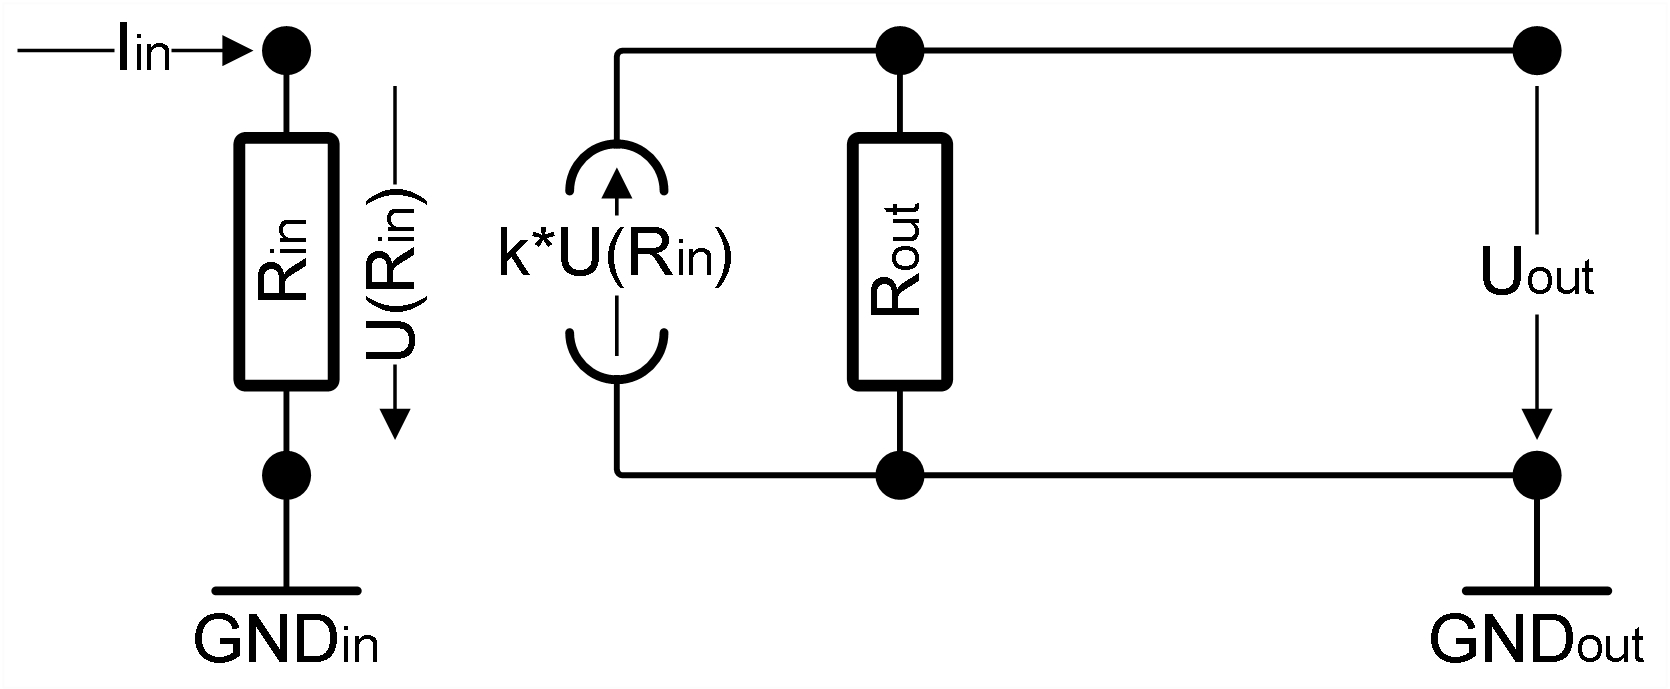
\includegraphics[width=5.38cm]{I2UConverter_I(u)}
\\

\end{tabular}
\caption{Current to voltage converter using a voltage controlled current source; $R_i=R_{in}$,
$R_o=R_{out}$}
\label{figI2UConverterUsingIByU}
\end{center}
\end{figure}
} % End of sample circuit: Voltage controlled current source

% End of list of figures of sample schematics used in the section.


\subsubsection{Passive device \code{R}, \code{Y}, \code{L}, \code{C}}

The passive devices resistor \code{R}, conductance \code{Y}, inductivity
\code{L} and capacitor \code{C} have two connectors and they are
independent of the chosen polarity. Just connect them by referencing two
nodes.

An example netlist can be found in section \ref{secIntro}; please refer to figure
\ref{figFirstIntroExample}, too.


\subsubsection{Constant voltage source \code{U}}

The constant voltage source \code{U} has two connectors. The plus and
minus pole of the source are the first and second referenced node,
respectively. The polarity is defined such that the first and second
referenced node designate the start and end of the arrow in the symbol of
the source (or voltage).

The given voltage of the source is an independent variable to the
computation but not considered a settable physical value; no value
assignment or device relation can be made in the definition of a constant
voltage source. The constant voltage appears as a variable in the
results.

At least one constant source, either voltage or current, needs to be
present in a computable netlist.

An example netlist is shown in figure \ref{figSimpleT}.


\subsubsection{Constant current source \code{I}}

The constant current source \code{I} has two connectors. The polarity is
defined such that the first and second referenced node designate the start
and end of the arrow in the symbol of the source: The current is flowing
into the network through the second referenced node and flowing back into
the source from the first referenced node.

The given current of the source is an independent variable to the
computation but not considered a settable physical value; no value
assignment or device relation can be made in the definition of a constant
current source. The constant current appears as a variable in the results.

At least one constant source, either voltage or current, needs to be
present in a computable netlist.

An example netlist is shown in figure \ref{figI2UConverterUsingUByI}.


\subsubsection{Current probe \code{PI}}
\label{secSyntaxCurrentProbe}

The current probe \code{PI} has two connectors and can be connected in
series with any other device to measure the current flowing through the
device. The sensed current becomes a new unknown, which can be
referenced in user-defined results.

The polarity of the measured current is defined such that the sensed
current is flowing into the probe from the first referenced node and
flowing back into the network through the second node.

A current probe is assumed an ideal wire. It has no physical value(s); no
value assignment or device relation can be made in the definition of a
current probe.

An example netlist is shown in figure \ref{figSimpleT}.


\subsubsection{Operational amplifier \code{OP}}

An operational amplifier \code{OP} has three connectors; connect them by
referencing three nodes.

The first two referenced nodes are the inputs. Different to real
circuits no distinction needs to be made between the two inputs; there's
no inverted or non inverted input. The computation needs to assume the linear
operation -- everytking else is out of scope of \linnet{} -- and in this
sense the connection is always made correct.

The third referenced node is the output of the op-amp.

Please note that the ground node needs to be explicitly defined if an
op-amp is used; see section \ref{secGndNode} for details.

An op-amp is assumed ideal. It has no output voltage or frequency limits
and hence no physical value(s); no value assignment or device relation can
be made in the definition of an op-amp.

An example netlist is shown in figure \ref{figNonInvOp}.


\subsubsection{Voltage controlled voltage source \code{U(U)}}

The voltage controlled voltage source \code{U(U)} has four connectors. The
actual source has two; these are the first two nodes referenced in the
device definition. The first node designates the positive pole of the
source, the second one the negative pole. First and second referenced
node designate start and end of the voltage defining arrow in the
schematic.

The control voltage is defined by the voltage potential difference between
node three and four, in this order. The third and forth referenced node
designate start and end of the voltage arrow in the schematic,
respectively.

An example netlist is shown in figure \ref{figModelOfOP}. Please note,
that the control voltage in this example is defined inverse to the input
voltage in order to model the inverting op-amp.


\subsubsection{Current controlled voltage source \code{U(I)}}

The current controlled voltage source \code{U(I)} has two connectors. The
first referenced node designates the positive pole of the source, the
second one the negative pole. First and second referenced
node designate start and end of the voltage defining arrow in the
schematic.

The control current is specified by a reference to a current probe. The
current probe is another, previously defined device (forward references
are not supported), which behaves like an ideal wire. The current through
this wire times the device constant of the controlled source is the
voltage enforced between the two referenced nodes. The reference to the
current probe is made by name; the name of the probe device follows the
pair of referenced nodes.

An example netlist is shown in figure \ref{figI2UConverterUsingUByI}.


\subsubsection{Voltage controlled current source \code{I(U)}}

The voltage controlled current source \code{I(U)} has four connectors. The
actual source has two; these are the first two nodes referenced in the
device definition. The second node designates the pole of the source,
which injects the current into the network. The same current flows back
into the source from the first referenced node. This way the first and
second referenced node designate start and end of the arrow in the symbol
of the source, respectively.

The control voltage is defined by the voltage potential difference between
node three and four, in this order. The third and forth referenced node
designate start and end of the voltage arrow in the schematic,
respectively.

An example netlist is shown in figure \ref{figI2UConverterUsingIByU}.


\subsubsection{Current controlled current source \code{I(I)}}

The current controlled current source \code{I(I)} has two connectors. The
second node designates the pole of the source, which injects the current
into the network. The same current flows back into the source from the
first referenced node. This way the first and second referenced node
designate start and end of the arrow in the symbol of the source,
respectively.

The control current is specified by a reference to a current probe. The
current probe is another, previously defined device (forward references
are not supported), which behaves like an ideal wire. The current through
this wire times the device constant of the controlled source is the
injected current. The reference to the current probe is made by name; the
name of the probe device follows the pair of referenced nodes.

An example netlist is shown in figure \ref{figSimpleT}.


\section{Result specification}
\label{secResultSpec}

The remaining parts of the file are used to specify the wanted results.
This part of the file may stay empty; now, there is one implicitly defined
result, a so called full result. It is named \ident{allDependends} and
contains the full set of dependencies of all unknown voltages and currents
on all known voltages and currents. Full results can easily become very
bulky (and practically useless) and should be avoided for all non trivial
circuits.

% TODO Equalize the inconsistent use of tags code and ident

Explicitly specified results consist of three elements, referred to by the
keywords \code{DEF}, \code{RES} \code{PLOT}. The first token behind these
keywords designates the name the specified object gets. This name must not
clash with any other name already in use, regardless whether it are names
of nodes or devices or if they have been introduced before by these
keywords. Furthermore, the internally derived names of unknowns need to be
avoided to. The current though a voltage source is e.g. derived from the
name of the source by prefixing it with \code{I\_}. Please refer to section
\ref{secModellingDevices} for a complete consideration.


\subsection{User-defined voltages}
\label{secUserDefVoltage}

The keyword \code{DEF} defines new voltages as difference of two nodes'
voltage potentials. Such a so called user-defined voltage is a new
explicitely defined unknown of the system. It doesn't matter if it is
identical to an already existing unknown voltage, then the same voltage
will be computed and reported twice with different names.

To give an example, we could extend our introductory example from section
\ref{secIntro}, figure \ref{figFirstIntroExample}, by adding the 
line

\begin{verbatim}
DEF U_c K1 out
\end{verbatim}

\noindent
to the netlist file. The first token behind keyword \code{DEF} is an
identifier, which gives a name to the new voltage. The two referenced
nodes follow. These nodes might be defined later; forward references are
allowed here.

Our example would add a user-defined voltage $U_c$ to the set of
unknowns that models the voltage drop at the capacitor.

There's no keyword for user-defined currents: If a specific current (e.g.
the current through the capacitor) should be put into the result then a
special, virtual device is applied, the current probe; please see section
\ref{secSyntaxCurrentProbe}.


\subsection{Full results}

If the set of user-defined voltages is complete then the keywords
\code{RES} and \code{PLOT} are applied to specify the result set. The
basic idea of both commands is to have dependent and independent
quantities and to present how the former depend on the latter.

The first token behind keyword \code{RES} is an identifier, which gives a
name to the new result. This name is used to title the found formulas in
the program output, and the generated Octave script that (numerically)
implements these formulas has the same name.

\code{RES} computes the full dependency of a set of unknown voltages or
currents on all known voltages and currents. (Known voltage and currents
are the device values of the constant voltage and current sources.) Since
the independents are always \emph{all} knowns of the system the command
only has the set of desired unknowns as parameter, as a blank separated
list of identifiers. Such an unknown can be a node's voltage potential,
the current through a voltage source or current probe, the output current
of an op-amp or a user-defined voltage. A complete list of knowns and
unknowns can be found in table \ref{tabUnknownsOfLES} on page
\pageref{tabUnknownsOfLES}.

In the Octave export this result is modeled as an LTI transfer function
object of kind MIMO (multiple inputs, multiple outputs). The default
operation of the generated script code is to plot a rectangular array of
step responses, where each sub-plot presents the step reponse of one
output if one but only one input undergoes a step and all others are
constantly null.

Extending our example so far, we could add the line

\begin{verbatim}
RES U_c_r U_c U_out
\end{verbatim}

\noindent
to our file \file{rlc.cnl}. The specification of result \code{U\_c\_r}
demands to compute the voltage drop at the capacitor and at the resistor.
The result specification builds on the previously made user-defined
voltage definition and exploits the fact that the voltage drop at the
resistor is identical to the voltage potential of network node \code{out};
the other end of the resistor is namely connected to the ground node.

Two formulas can be expected. Both voltages will depend on the input
voltage, which is the only independent quantity of the system. An LTI
transfer function object of kind SIMO with one input and two outputs will
be created by the generated Octave script \file{rlc/U\_c\_r.m}. 


\subsection{Bode plots and inverse transfer functions}

The keyword \code{PLOT} specifies a result with exactely one independent
and one dependent voltage or current. This is normally one of the partial
transfer functions of a full result as specified with \code{RES}. The
default operation of the generated Octave script is to open the Bode plot
of this transfer function, which is the most common operation having such a
transfer function.

The first token behind keyword \code{PLOT} is an identifier, which gives a
name to the new result. This name is used to title the found formula in
the program output, and the generated Octave script that (numerically)
implements this formula has the same name.

\code{PLOT} is not just a sub-set of \code{RES}. Its added value is the
larger freedom in chosing the dependent and independent quantity of the
plot. The dependent quantity can be an actually given, known quantity,
whereas the independent quantity can be an unknown to the internal
computation. This permits to compute and plot inverse transfer functions.
The most important use case is the computation of the input impedance of a
circuit: The (known) input voltage is plotted in dependence on the
(unknown) input current.

Even two unknowns can serve as a pair of independent and dependent
quantity. Now, the transfer function shows how these two unknowns are
related to each other if the input voltage is modulated. This mode is
restricted to single input circuits, otherwise the relation wouldn't be
unambiguous.

Refering to two known quantities is forbidden.

If we have the unknown $u$, which depends on the known $k$ and if
$k$ is the only known of the system then the result specification
\code{PLOT R u k} leads to the same computation as \code{RES R u}
would. The only difference is the selected default operation in the Octave
export: Using \code{PLOT} we get a Bode transfer function plot, using
\code{RES} we get the step response. However, the generated LTI object is
exactely the same; in either case you can get the other plot, too. It just
needs a few more key strokes inside Octave.

In our introductory example we had used the line

\begin{verbatim}
PLOT G U_out U_in
\end{verbatim}

\noindent
to specify the result \code{G}, which means the SISO system's transfer
function, the dependency of its single output on its single input. The
result specification refers to the voltage potentials of the in- and
output node, which is suitable as the other, negative end of the in- and
output voltage definitions is the ground node.

A list of the knowns and unknowns, which can be referenced from a
\code{PLOT} result specification can be found in table
\ref{tabUnknownsOfLES} on page \pageref{tabUnknownsOfLES}.


\subsection{Plot control}

The generated Octave script code defaults to some initial plots. (Using
the created LTI transfer function objects any other arbitrary plots and
figures can be created in Octave.) These initial plots can be controlled
in a rather limited way from the netlist file with some additional syntax
elements.

A line starting with either \code{RES} or \code{PLOT}, which specifies a
result, may be continued -- after some separating white space -- with a
``plot-info'' block. The plot-info begins with the keyword \code{LIN} for
a plot with linear frequency axis or \code{LOG} for a logaritmic axis. An
integer number follows up. It indicates the number of points computed for
and displayed in the plot. For linear frequency axes this is the total
number of points whereas for logarithmic axes it is the number of points
per decade. The plot-info (and the result specification) is closed with a
pair of positive floating point numbers, which designates the frequency
range of the plot in Hz.\footnote{Hz is a convenient unit to specify the
desired frquency range but it can be confusing as Octave's frequency axis
is scaled in rad/s; the displayed numeric range will differ by $2 pi$ from
your input.}

If the default plot is a time domain plot (as for full results) then the
plot-info still relates to the (actually not presented) Bode transfer
function plot of the system. The according range of the time variable of
the actual plot is derived from this information. Basically, the upper
limit of the time range is the reciprocal of the upper limit of the
specified frequency range.

If the optional plot-info block is not used then \linnet{} won't pass any
plot related information on to Octave. Most of the Ocatve functions from
the control toolbox will safely find suitable ranges for plotting
themselves so that this normally is the simplest and best way to do.


\section{Ground nodes}
\label{secGndNode}

A valid network of devices may consist of any number of unconnected
sub-networks. (It's probably hard to find reasonable uses cases for
unconnected sub-nets with maybe the exception of sub-nets coupled by
controlled sources.) \linnet{} assumes an unknown voltage potential for
each but one of the sub-network nodes; the last voltage potential is
linear dependent inside a sub-network. The excluded nodes are called the
ground nodes and their voltage potential is null by definition. Normally
\linnet{} will select suitable ground nodes for you and the final results
won't depend on this selection.

If you want to define the ground node of a sub-network yourself you can do
this by naming. If there's one node whose name contains either ``gnd'' or
``ground'', either capitalized or in all lower or all upper case, then
this node will become the ground node. If two or more nodes have such a
name within the same sub-network then the computation is refused.

The explicit choice of a ground node is often advantageous to simplify the
result specification. The voltage potentials of all nodes but the ground
nodes can be referenced by name in the result specification. If you define
your circuit such that system in- and output voltage are the voltage
difference between an in- and output node and a common other node then
you'd preferrably define this common node as ground node - system in- and
output voltage are now directly accessible as node voltage potentials. If
you leave the choice of the ground node to \linnet{} or if you'd make
another node the ground node then you had to define the system in- and
output voltages explicitly as potential differences using the keyword
\code{DEF}, please see section \ref{secUserDefVoltage} for details.

The definition of the ground node is no longer a matter of convenience
only but directly impacts the computation result if you use at least one
operational amplifier in a sub-network. Op-amps are modeled as controlled
voltage sources connected to the ground node, this is why. If an op-amp is
used then \linnet{} can no longer decide autonomously which node to take
as ground node - it can't guess your intentions. You have to define the
ground node explicitly, the computation is refused otherwise.

It's natural and considered good practice to always define the ground
nodes of a circuit explicitly.


\section{The deprecated netlist format \code{*.ckt}}

The parser of \linnet{} still supports an elder, deprecated input format.
It had been used by an initial, much simpler implementation of the core
algorithm, which had served as prove of concept. It had limited
capabilities and its netlist syntax, which followed the SPICE netlist
format could not easily be extended to express the features of the
\linnet{} release. Furthermore the similarity with the SPICE syntax turned
out to be rather disadvantageous as it promised much more compatibility
as could ever be kept due to the different concepts of the programs.

The \file{*.ckt} input format has been retained for regression testing
only; the \linnet{} release should yield the same results as the prove of
concept. It is not intended to support this format in future releases and
you're not encouraged to ever use it. This is why it is not explained in
this manual. A formal syntax description in Backus-Naur form can however
be found as \file{parser-ckt-bnf.txt}. The file is part of the \linnet{}
sources.
